\documentclass[10pt]{article}

%%%%%%%%%% CONFIGURACIÓN DE PÁGINAS %%%%%%%%%%%%%%%
\usepackage[text=17cm,
	    left=2cm,
	    right=2cm, 
	    headsep=20pt, 
	    top=2.5cm, 
	    bottom = 2.5cm,
	    onecolumn,
	    twoside,
	    letterpaper,
	    asymmetric,
	    showframe = false]{geometry} 

\usepackage{latexsym,amsmath,amssymb,amsfonts,amsthm} %(símbolos de la AMS)
\usepackage[T1]{fontenc} %acentos en español
\usepackage[utf8]{inputenc} % eñes y tildes
\usepackage{paracol} % texto en columnas
\columnratio{0.6,0.4} % 60% de la página para la columna 1 y 40% para la columna 2
\setlength{\columnsep}{1cm} % Ajusta el espacio entre las columnas a 1cm
\usepackage{graphicx} % Incluir imágenes
\usepackage{tikz} % Dibujos con código
\usepackage{sectsty} % Cambiar el estilo de los títulos
\usepackage{fancyhdr} % Encabezados y pies de página
\usepackage[spanish]{babel} % Español
\usepackage{natbib} % Referencias bibliográficas
\usepackage{titlesec}
\titlespacing*{\section}{0pt}{10.5ex plus 1ex minus .2ex}{4.3ex plus .2ex}


\definecolor{pastelblue}{rgb}{0.0667, 0.5529,1}
\allsectionsfont{\color{pastelblue}} % Aplica el color azul pastel a todos los títulos

\begin{document}

% Tipo de letra
\fontfamily{pnc}\selectfont

\pagecolor{blue!30!black!20!}
% Carátula
\begin{titlepage}
    \centering
    %\includegraphics[width=0.5\textwidth]{tu_logo.png} % Agrega tu logo o imagen aquí
    \vspace{2cm}
    
    {\Huge\bfseries Reporte\par}
    \vspace{1cm}
    
    {\Large por: Christian L. Paredes Aguilera\par}
    \vspace{4.5cm}

    
\includegraphics[width=0.7\textwidth]{../image/logo.png}

    
    \vfill
    {\large San miguel, calle Enrique Peñaranda 34, Edificio NV\par}
    {\large Celular: +59170174745\par}
    {\large Correo: info@altitudesolutions.org\par}
    {\large Fecha: \today\par}
\end{titlepage}

\pagecolor{white}

\tableofcontents
\listoffigures
\listoftables

\newpage
\begin{paracol}{2}
\section*{Análisis descriptivo del conjunto de datos}
Las tablas contienen un total de 10.001 registros, lo que indica una cantidad considerable de datos para el análisis. También contienen 9 columnas que representan diferentes variables, incluyendo la región, el país, el tipo de producto, la fecha de pedido, el ID de pedido, la fecha de envío, las unidades totales vendidas, el precio unitario en dólares estadounidenses y el costo total en dólares. En cuanto a los datos numéricos, aquí hay algunos puntos destacados:

\begin{itemize}
    \item Unidades Totales Vendidas: El número medio de unidades vendidas es de 5.002, con un mínimo de 2 y un máximo de 10.000 unidades.
    \item Precio Unitario (\$us): El precio unitario promedio es de \$268,14, con un mínimo de \$9,33 y un máximo de \$668,27.
    \item Costo Total (\$us): El costo total promedio es de \$938.172, con un mínimo de \$30,87 y un máximo de \$5.241.726.
    \item Precio Total (\$us): El precio total promedio es de \$1.333.222, con un mínimo de \$167,94 y un máximo de \$6.680.027.
    \item Costo Unitario (\$us): El costo unitario promedio es de \$188,79, con un mínimo de \$5,14 y un máximo de \$524,96.
\end{itemize}

Estos datos proporcionan una visión general de las ventas y los costos asociados a los productos. Para un análisis más detallado, podríamos considerar agrupar los datos por región, país o tipo de producto, o analizar las tendencias a lo largo del tiempo utilizando las fechas de pedido y envío.
\newpage

\switchcolumn[1]*{\noindent\scriptsize
    \begin{figure}
	\centering
	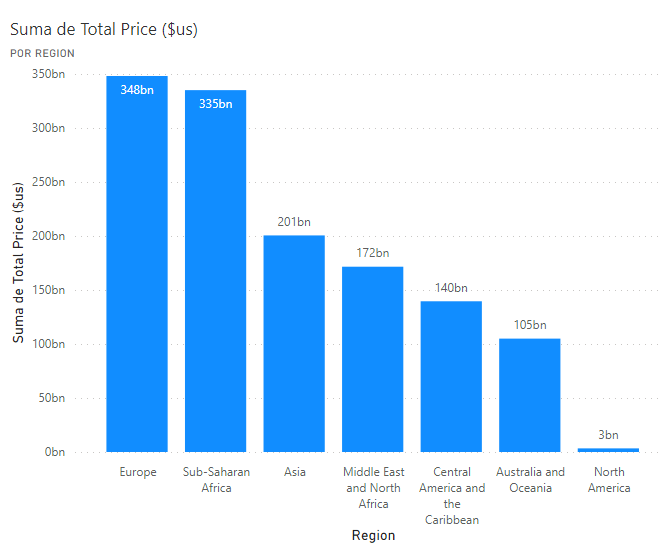
\includegraphics[width=0.4\textwidth]{../image/uno.png}
	\caption{Ventas totales en diferentes regiones del mundo}
    \end{figure}
}
\switchcolumn[0]\noindent

\section{¿Qué región tiene las ventas más altas (en \$us) y con cuánto?}
El análisis de las ventas totales en diferentes regiones del mundo revela, según la figura 1, que \textbf{Europa} lidera con ventas de \$3.481 billones. Le sigue Asia con ventas significativas de \$2.005 billones. Centroamérica y el Caribe también muestran un fuerte rendimiento con \$1.395 billones en ventas. Australia y Oceanía, por otro lado, registran ventas de \$1.049 billones. A pesar de estas cifras impresionantes, es importante notar que América del Norte muestra las ventas más bajas con \$353.5 mil millones. Estos datos proporcionan una visión valiosa de las tendencias de ventas globales y pueden ser útiles para informar estrategias de mercado y de ventas futuras.

\section{¿Qué país tiene la mayor cantidad de unidades de carne vendidas?}
\switchcolumn[1]{\noindent\scriptsize
    \begin{figure}
	\centering
	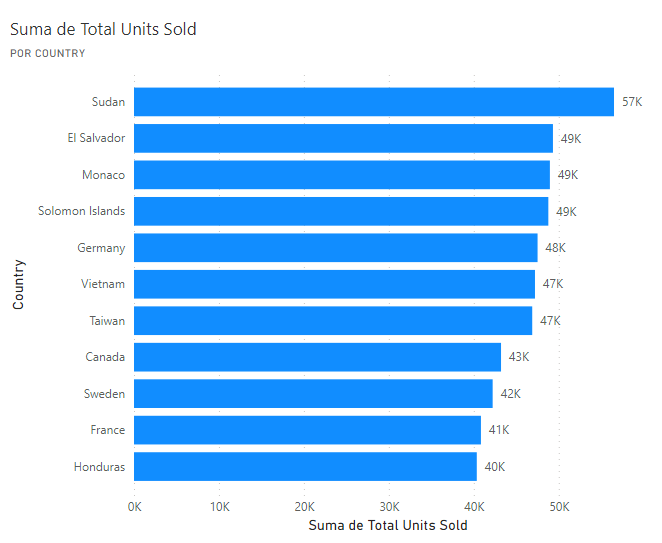
\includegraphics[width=0.4\textwidth]{../image/dos.png}
	\caption{Mayor cantidad de unidades de carne vendidas por país}
    \end{figure}
}
\switchcolumn[0]\noindent
Según la figura 2, \textbf{Sudán} tiene el mayor número de unidades vendidas con 56.503, lo cual es significativamente mayor que el número de unidades vendidas en otros países. El Salvador y Mónaco siguen de cerca a Sudán con 49.315 y 48.955 unidades vendidas respectivamente. 

\section{Dato inconsistente}

\switchcolumn[1]{\noindent\scriptsize
    \begin{figure}
	\centering
	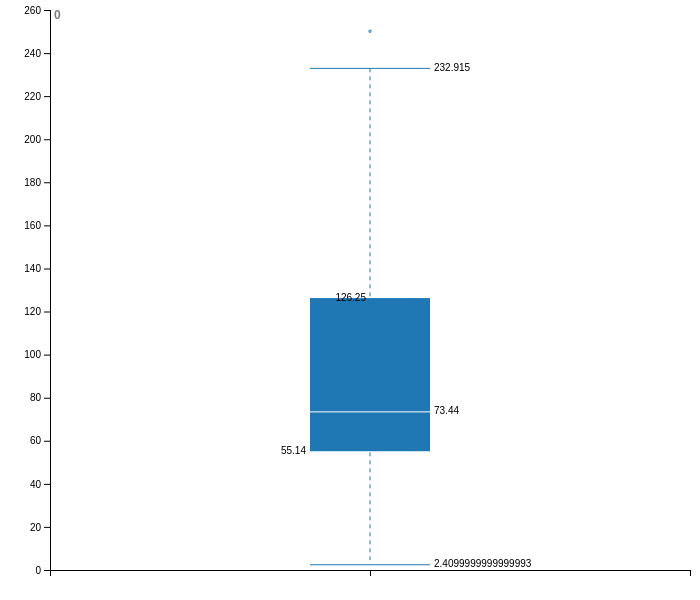
\includegraphics[width=0.4\textwidth]{../image/tres.png}
	\caption{Dato inconsistente en el margen bruto unitario}
    \end{figure}
}
\switchcolumn[0]\noindent
Dado al supuesto inicial :"Todos los productos dentro de un tipo de producto (product type) generan el mismo margen bruto unitario en todos los países." Se busco el dato atípico al calcular el margen bruto unitario porcentual \footnote{Se recomienda usar el margen bruto sobre las ventas, que da paso a una medida porcentual}. De todas formas, se realizó el calculo del margen bruto unitario en \$us con el propósito de compararlo con el calculo del margen bruto unitario porcentual.

Esta comparación se hizo mediante el método de \cite{tukey1949} denominado, del Rango Intercuartil (IQR)  \footnote{El método del Rango Intercuartil (IQR) funciona bien en distribuciones diferentes a la normal}. Y verificado con la Figura 3, que corresponde a un gráfico Boxplot.

Durante el proceso al utilizar el margen bruto unitario en términos porcentuales, se identificaron 873 observaciones atípicas. Entre estas, una en particular destacó por su considerable desviación respecto a la media. En cuanto al margen bruto unitario (\$us), se detectó únicamente una observación atípica, que coincide precisamente con la observación extremadamente desviada identificada en el cálculo porcentual. Esta observación corresponde a:
\begin{table}[h]
\centering
\begin{tabular}{|l|l|l|}
\hline
\textbf{Region} & \textbf{Country} & \textbf{Product Type} \\
    Europe & \textbf{Spain} & Baby Food \\
\hline
\end{tabular}
\caption{Dato inconsistente}
\end{table}


\section{¿Cuál es el tipo de producto con mayor margen bruto porcentual?}
\switchcolumn[1]{\noindent\scriptsize
    \begin{figure}
	\centering
	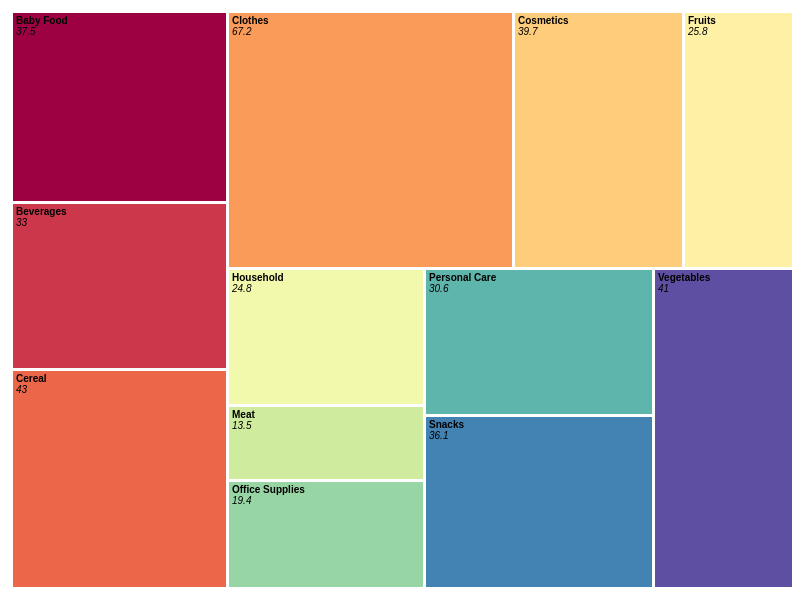
\includegraphics[width=0.4\textwidth]{../image/cuatro.png}
	\caption{TreeMap de margen bruto porcentual por tipo de producto}
    \end{figure}
}
\switchcolumn[0]\noindent
De acuerdo con la figura 4, se observa que el producto \textbf{Clothes} presenta el margen bruto porcentual más elevado, con un valor de 67.2\%. En contraste, el producto \textit{Meat} exhibe el margen bruto porcentual más reducido, con un valor de 13.5\%. Estos hallazgos son específicos para los datos contenidos en la tabla proporcionada y pueden variar con diferentes conjuntos de datos o condiciones del mercado.



\section{Grafica un pareto de margen bruto por país e indica cuántos países cubren el \boldmath $80\%$ del margen generado a nivel mundial.}
\switchcolumn[1]{\noindent\scriptsize
    \begin{figure}
	\centering
	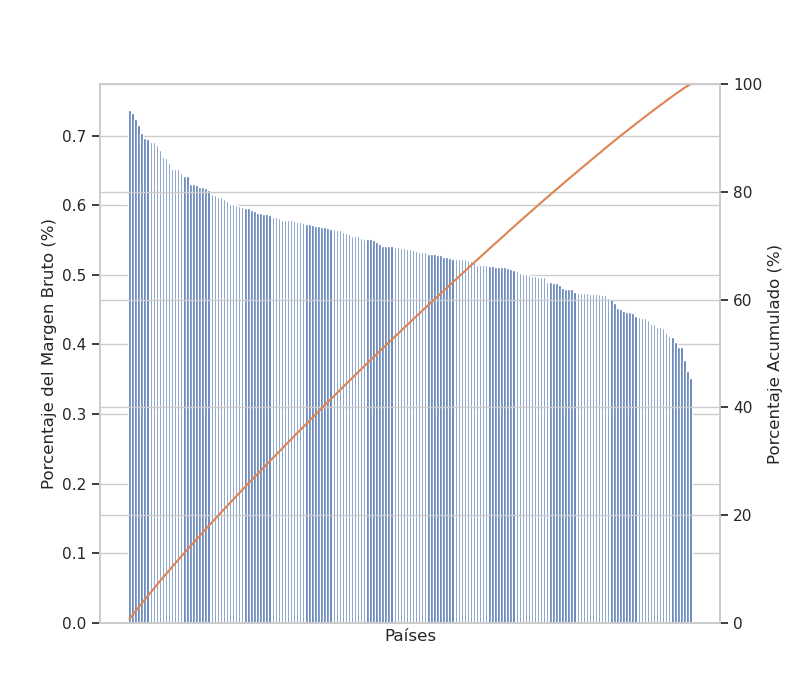
\includegraphics[width=0.4\textwidth]{../image/cinco2.png}
	\caption{Pareto de margen bruto porcentual por país}
    \end{figure}
    \begin{figure}
	\centering
	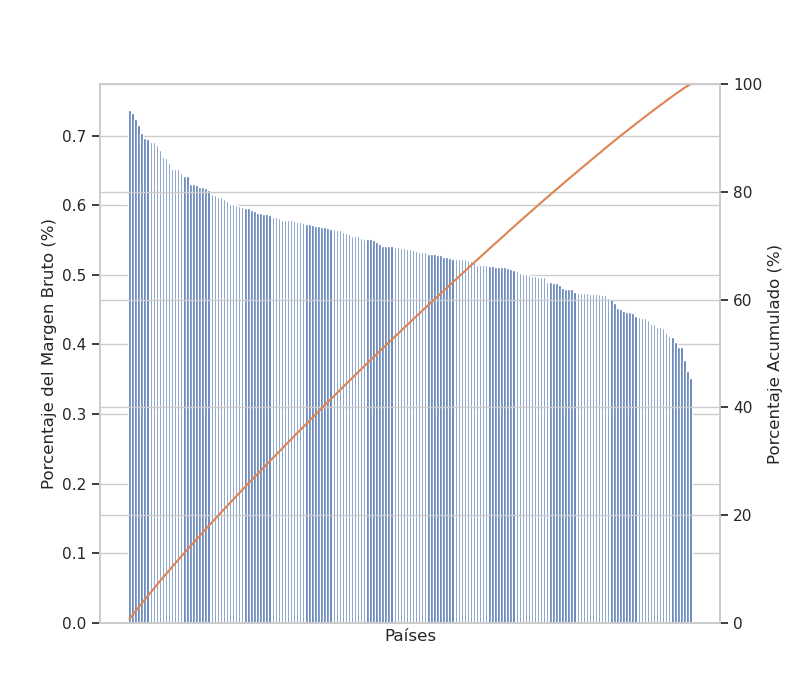
\includegraphics[width=0.4\textwidth]{../image/cinco1.png}
	\caption{Pareto de margen bruto monetario (\$us) por país}
    \end{figure}
}
\switchcolumn[0]\noindent
De igual manera como en la sección 3.3, se realizó los cálculos del margen bruto por país en términos porcentuales y en términos de monetarios (\$us). Para luego según
\cite{grosfeld2007}, esbozar los gráficos de Pareto.

Observemos, que aún tendría sentido utilizar datos en términos porcentuales para el gráfico de Pareto, ya que el margen bruto porcentual es una medida más útil para comparar el rendimiento de diferentes países. Por otro lado, utilizar el margen bruto en \$us para el gráfico de Pareto, nos proporcionará una medida más directa del rendimiento financiero.

Para el caso del \textbf{margen bruto porcentual}, se observa que el $80\%$ del margen bruto por país es generado por \textbf{140 países} (Figura 5). Mientras que para el margen bruto monetario (\$us), el $80\%$ del margen bruto por país es generado por \textbf{137 países} (figura 6).


\section{Calcula el tiempo promedio (en días) por país que toma en ser enviada una orden desde la fecha en que se registra la orden (order date vs ship date)}
\switchcolumn[1]{\noindent\scriptsize
    \begin{figure}
	\centering
	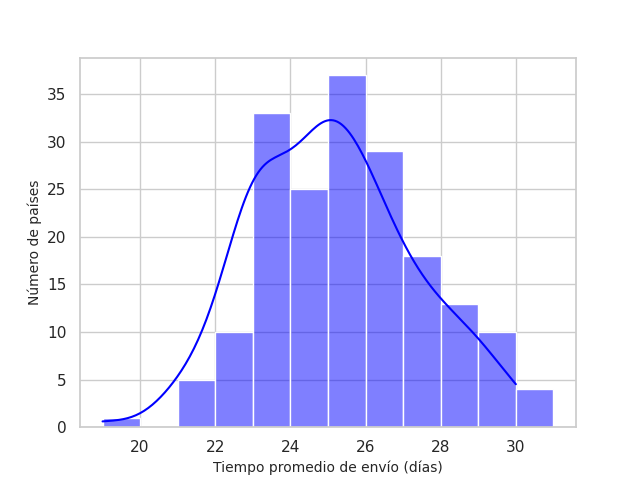
\includegraphics[width=0.4\textwidth]{../image/seis.png}
	\caption{Histograma de tiempo promedio por país}
    \end{figure}
}
\switchcolumn[0]\noindent
En el análisis de los tiempos promedio de envío, se ha identificado que \textbf{Yemen} es el país con el menor tiempo promedio, registrando un total de \textbf{19 días}. Este dato es relevante para entender la eficiencia del proceso de envío en Yemen.

Además, al visualizar estos tiempos promedio a través de un \textbf{histograma} de la Figura 7, con un rango de contenedores (bins) de 1 día, se ha encontrado que el \textbf{rango} que incluye la mayor cantidad de países es de \textbf{25 días}. Este hallazgo es crucial para entender las tendencias globales en los tiempos de envío.


\section{Calcula la tasa de crecimiento anual compuesta de ventas a nivel mundial, para el mayor rango de años consecutivos con ventas en todos los meses del año.}
La Tasa de Crecimiento Anual Compuesta (TCAC), también conocida como CAGR (Compound Annual Growth Rate), se calcula utilizando la siguiente fórmula:
$$
CAGR = \left( \frac{EV}{BV} \right)^{\frac{1}{n}} - 1
$$
donde:
\begin{itemize}
    \item $EV$ es el valor final,
    \item $BV$ es el valor inicial, y
    \item $n$ es el número de años.
\end{itemize}
\vspace{0.2cm}
Aplicando esta formula al análisis de ventas a nivel mundial, se calculó para el mayor rango de años consecutivos en todos los meses del año. Este rango se extendió desde el \textbf{año 2010 hasta el año 2016}.

El resultado del análisis mostró que la \textbf{TCAC} para este período fue del \textbf{1.25\%}. Este valor representa la tasa constante a la que habrían crecido las ventas si hubieran crecido al mismo ritmo cada año durante este período de tiempo


\section{Para órdenes realizadas (order date) en diciembre del 2015, responde a las siguientes preguntas utilizando una tabla dinámica:}

\begin{table}[h]
    \centering
    \begin{tabular}{|l|c|}
	\hline
	\textbf{Día} & \textbf{N Ordenes} \\
	\hline
	Sunday & 13 \\
	\hline
	Monday & 27 \\
	\hline
	Tuesday & 12 \\
	\hline
	Thursday & 19 \\
	\hline
	Friday & 10 \\
	\hline
	Saturday & 21 \\
	\hline
    \end{tabular}
    \caption{Ordenes realizadas en diciembre del 2015, por día de la semana}
\end{table}


\paragraph{Identifica en qué día de la semana (lunes - domingo) se dan la mayor cantidad de envíos}.
Según la Tabla 2, se identificó que el \textbf{lunes} es el día de la semana en el que se realizan la mayor cantidad de envíos. Este hallazgo es crucial para entender los patrones de envío y puede ser útil para optimizar las operaciones de logística y distribución. 

\paragraph{Identifica en qué día de la semana (lunes-domingo) se dan la menor cantidad de envíos}.
Según la Tabla 2, se identificó que el \textbf{viernes} es el día de la semana que registra la menor cantidad de envíos. Este hallazgo puede ser útil para optimizar las operaciones y recursos de la empresa durante la semana. 

\end{paracol}

\bibliography{biblio}
\bibliographystyle{apalike}

\end{document}
